\section{Representing a Ring of Sets by Set Differences}

In this section we continue our examination of a general ring of sets $\mathcal{F}$, focusing on the set differences between elements of $\mathcal{F}$. We will then use certain set differences to define a new representation of $\mathcal{F}, D(\mathcal{F})$, that will be more useful than $I(\mathcal{F})$ for algorithmic purposes, and in the case of the stable marriage problem, can be more efficiently constructed than $I(\mathcal{M})$.

\subsection{The Centers of a Ring of Sets}

The unique minimal element of a ring of sets $\mathcal{F}$ will be called the zero of $\mathcal{F}$, and will be denoted by $F_0$. For an irreducible element $F$ of $\mathcal{F}$, the center of $F$, written $K(F)$, is the set $\{a \in B: F(a)=F\}$. Note that the center of an element $F$ is defined only if $F$ is irreducible. Note also that $K\left(F_0\right)=F_0$. but for any other irreducible element $F, K(F) \subset F$, since $F_0 \subset F$. In each irreducible element $F$ of $\mathcal{F}$, shown in Figures \ref{FIG_2_5} and \ref{FIG_2_6} , the elements of $B$ in the center of $F$ are underlined. So, for example, the center of $F_2$ is $\{d, e\}$.

\begin{lemma}\label{lem_2_8}
 Every element of $B$ is a member of at most one center of $\mathcal{F}$.
\end{lemma}

\begin{proof}
    If $a \in K\left(F_i\right) \cap K\left(F_j\right)$, then $F_i=F(a)=F_j$.
\end{proof}

\subsection{The centers represent a ring of sets}
 
 Just as every element $F \in \mathcal{F}$ can be expressed as the union of the irreducible elements that precede it in $\mathcal{F}, F$ can also be expressed as the union of the centers of the irreducible elements that precede $F$ in $\mathcal{F}$. This provides a more revealing and economical expression for $F$, since distinct centers never intersect. 
\begin{lemma}\label{lem_2_9}
    For any element $F$ in $\mathcal{F}, F=\bigcup\left\{K\left(F_i\right): F_i \in U(F)\right\}$. Further, this is the only way to express $F$ as the union of a set of centers of $\mathcal{F}$.
\end{lemma}

\begin{proof}
     By definition of $U(f), F(a)$ is in $U(F)$ for every $a$ in $F$. Also, $a$ must be in $K(F(a))$, which is a subset of $F(a)$. It follows then that $F \subseteq \bigcup\left\{K\left(F_i\right): F_i \in U(F)\right\}$. Conversely, for every $F(a) \in U(F), F(a)$ is a subset of $F$, so $K(F(a))$ is a subset of $F$, and hence $\left\{K\left(F_i\right)\right.$ : $\left.F_i \in U(F)\right\} \subseteq F$. The uniqueness of the expression follows from the fact that no distinct centers intersect.
\end{proof}

We now define $D(\mathcal{F})$ to be the set of all centers of $\mathcal{F}$ other than $F_0$. The set $D(\mathcal{F})$ will allow us to focus on and characterize the minimal differences between elements of $\mathcal{F}$. These differences will serve as building blocks to construct and represent $\mathcal{F}$. We begin to make this precise with the following immediate corollaries of Lemma \ref{lem_2_9}.


\begin{corollary}\label{cor_2_3}
For any distinct elements $F_i$ and $F_j$ in $\mathcal{F}$, the symmetric difference of $F_i$ and $F_j,\left(F_i \backslash F_j\right) \cup\left(F_j \backslash F_i\right)$, is the union of a set of centers in $D(\mathcal{F})$. Further, there is only one set of centers whose union is the symmetric difference of $F_i$ and $F_j$.
\end{corollary}

\begin{exmp}\label{exmp_2_8}
    The symmetric difference of $F_8$ and $F_{11}$ shown in Figure \ref{FIG_2_5} is $\{c, f, g, h, i\}$, which is the union of $\left\{K\left(F_1\right), K\left(F_3\right), K\left(F_5\right), K\left(F_{11}\right)\right\}$, as may easily be verified.
\end{exmp}

\begin{corollary}\label{cor_2_4}
    If $F_0$ and $F_z$ are respectively the minimal and maximal elements of $\mathcal{F}$, then $F_z \backslash F_0$ is the union of all the centers in $D(\mathcal{F})$. i.e., $F_z \backslash F_0=\bigcup\left\{K\left(F_i\right): F_i \in I(\mathcal{F}) \backslash F_0\right\}$.
\end{corollary}

The following Lemma is a partial converse to Corollary \ref{cor_2_3}.

\begin{lemma}\label{lem_2_10}
    Every center $K(F)$ in $D(\mathcal{F})$ is the symmetric difference of a pair of elements of $\mathcal{F}$. In fact, $K(F)=F \backslash \hat{F}$, where $\hat{F} \subset F$ is an element of $\mathcal{F}$.
\end{lemma}

\begin{proof}
    Let $F$ be any nonzero element of $I(\mathcal{F})$, and let $\hat{F}$ be the union of all elements of $\mathcal{F}$ that strictly precede $F$. Clearly, $\hat{F}$ is an element of $\mathcal{F}$, and $\hat{F} \subset F$, so $F \backslash \hat{F}$ is a symmetric difference of a pair of elements of $\mathcal{F}$. Further, it follows easily from the definition of $K(F)$ that $F \backslash \hat{F} \subseteq K(F)$, and $K(F) \subseteq F \backslash \hat{F}$, so $F \backslash \hat{F}=K(F)$.
\end{proof}

\subsection{The minimal differences of $\mathcal{F}$}


Lemma \ref{lem_2_10} and Corollary \ref{cor_2_3} establish that the elements of $D(\mathcal{F})$ are precisely the minimal elements, with respect to set containment, of the set of all symmetric differences of distinct elements in $\mathcal{F}$. That is, every symmetric difference of a pair of elements in $\mathcal{F}$ is the union of a set of centers in $D(\mathcal{F})$, and every element in $D(\mathcal{F})$ is the symmetric difference of a pair of elements of $\mathcal{F}$. This view of $D(\mathcal{F})$ will be essential, and in order to emphasize the connection of $D(\mathcal{F})$ to set differences, we will hereafter refer to a center of $F \in D(\mathcal{F})$ as a minimal difference of $F$ and use the notation $D(F)$ in place of $K(F)$. The set $D(\mathcal{F})$ will be called the set of minimal differences of $\mathcal{F}$.

\subsection{The Partial Order of Minimal Differences}
Given the close connection between the sets $D(\mathcal{F})$ and $I(\mathcal{F})$, and the fact that the nonempty closed subsets of $I(\mathcal{F})$ represent $\mathcal{F}$, it should not be surprising that the closed subsets of $D(\mathcal{F})$ can also be used to represent $\mathcal{F}$ as we now show.

We define $(D(\mathcal{F}), \preceq)$ to be the partial order on the set $D(\mathcal{F})$ obtained by removing $F_0$ from the partial order $I(\mathcal{F})$ and then replacing each remaining element $F \in I(\mathcal{F})$ by its associated minimal difference $D(F)$. The precedence relation $(\preceq)$ on $D(\mathcal{F})$ is inherited from the precedence relation on $I(\mathcal{F})$ (and hence from $\mathcal{F}$): $D(F)$ precedes $D\left(F^{\prime}\right)$ in $(D(\mathcal{F}) \preceq)$ if and only if $F$ precedes $F^{\prime}$ in $I(\mathcal{F})$, i.e., $F \subseteq F^{\prime}$. In other words, the partial order $D(\mathcal{F})$ is isomorphic to the partial order $I(\mathcal{F})$ after the removal of the unique minimal element from $I(\mathcal{F})$. Figure \ref{FIG_2_8} shows the representation $D(\mathcal{F})$ obtained from $I(\mathcal{F})$ of Figure \ref{FIG_2_6}.

Now each minimal difference is associated with exactly one element of $I(\mathcal{F})$, and the precedence relation on $D(\mathcal{F})$ agrees with the relation on $I(\mathcal{F})$, so there is a one-one correspondence between the non-empty closed subsets of $I(\mathcal{F})$ and the closed subsets (including the empty subset) of $D(\mathcal{F})$; the closed subset of $I(\mathcal{F})$ consisting of $F_0$ corresponds to the empty subset of $D(\mathcal{F})$. Given the one-one correspondence between the elements of $\mathcal{F}$ and the nonempty closed subsets of $I(\mathcal{F})$ , the following is immediate.
%\newline
%\pagebreak

\begin{theo}
There is a one-one correspondence between the elements of $\mathcal{F}$ and the closed subsets of $D(\mathcal{F})$. Further, if $F_i$ and $F_j$ are elements in $\mathcal{F}$ corresponding to closed subsets $D_i$ and $D_j$ of $D(\mathcal{F})$, then $F_i \subset F_j$ if and only if $D_i \subset D_j$
\end{theo}

\begin{figure}[h]
  \centering
  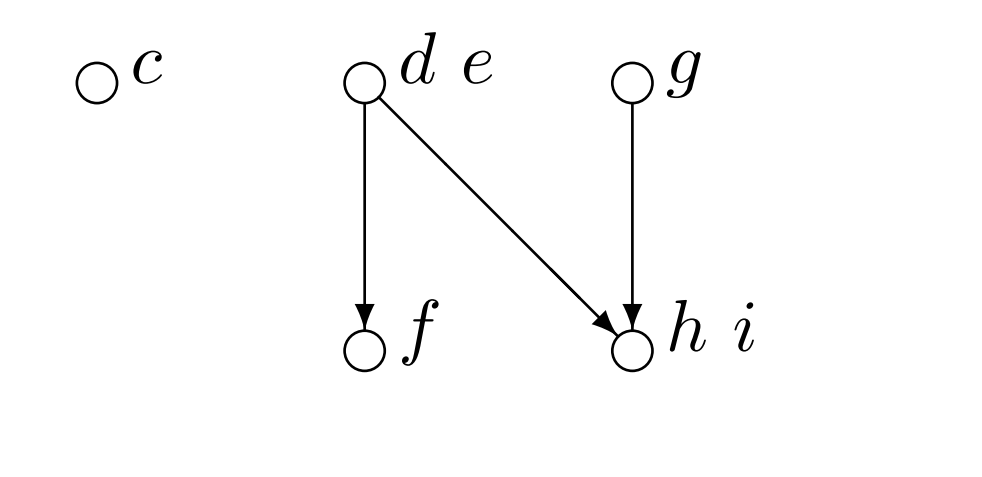
\includegraphics[width=0.5\textwidth]{IMAGES_FIGS/FIG_2_6.png}
  \caption{The partial order $D(\mathcal{F})$ for $\mathcal{F}$}
  \label{FIG_2_8}
\end{figure}